\begin{frame}
	\setbeamercolor{block body}{bg = yellow}
	\begin{block}{}
		\begin{center}
			{\large\textbf{Corso di base JAVA}}\\
			\itshape{Mauro Donadeo}\\
			mail: mauro.donadeo@gmail.com
		\end{center}
	\end{block}
	\setbeamercolor{block body}{bg = white}
	\begin{block}{}	
		\begin{center}
			\large{INTRODUZIONE}\\
			
\includegraphics[width = 30mm]{images/java-logo.jpg}
		\end{center}
	\end{block}	
\end{frame}

\section{Informazioni generali}
\subsection{Corso}
\begin{frame}
\frametitle{Informazioni generali}
\begin{block}{Orari lezioni}
\begin{itemize}
\item Martedì 27 marzo {\itshape ore 13:30 - 18:30};
\item Mercoledì 28 marzo {\itshape ore 14:00 - 19:00};
\item Venerdì 30 marzo {\itshape 9:30 - 13:30};
\item Martedì 3 aprile {\itshape 13:30 - 18:30};
\item Giovedì 5 aprile {\itshape 13:30 - 18:30};
\end{itemize}
\end{block}
\begin{block}{Dove}
Tutte le lezioni si svogeranno all'interno dell'aula CAR.
\end{block}
\end{frame}

\subsection{About me}
\begin{frame}
\frametitle{About me}
\begin{block}{}
Laureato in ingengeria informatica ad ottobre del 2011. Titolo della
tesi: \textit{Realizzazionde di un sistema di video conferenza 3D utilizzando 
il sistema di video conferenza MS Kinect}.
\end{block}

\begin{block}{Posizione attuale}
\begin{itemize}
\item Collaboro con il Prof. Gamberini all'interno di HTLab (htlab.psy.unipd.it);
\item Gesture recognition su dispositivi touchless all'inteno del progetto europeo
CEEDs (ceeds-project.eu);
\item Misure di accuracy di più Kinect che funzionano contemporaneamente. Sempre con 
il fine di riconoscere gesture.
\end{itemize}
\end{block}
\end{frame}

\section{Cos'è un programma}
\begin{frame}
\frametitle{Cos'è un programma}
\begin{block}{Il computer}
Tutti sappiamo che un computer è una macchina che: 
\begin{itemize}
\item \textbf{memoriza dati} (numeri, parole, immagini suoni...);
\item \textbf{interagisce con dispositivi} (schermo, tastiere, mouse, kinect...)
\item \textbf{esegue programmi}.
\end{itemize}
\end{block}
\pause
\begin{block}{I programmi}
I programmi sono \textbf{sequenze} di \textit{istruzioni} che il \textbf{computer}
\textit{esegue}, e di \textit{decisioni} che il \textbf{computer} prende per svolgere
una certa attività.
\end{block}
\end{frame}
\subsection{Cos'è un programma}
\begin{frame}
\begin{block}{}
Nonostante i programmi sono molto sofisticati e svolgano funzioni molto complesse, le 
istruzioni di cui sono composti sono \textbf{molto elementari} per esempio:
\begin{itemize}
\item estrarre un numero da una posizione di memoria;
\item inviare un documento in stampa;
\item accendere un punto rosso in una pos. determinata dello schermo;
\item se un numero è negativo, allora si svolge una funzione più tosto che un altra.
\end{itemize}
\end{block}
\begin{block}{Programmazione}
Un programma descrive al computer in estremo dettaglio la sequenza necessaria di 
passi per svolgere un particolare compito:
\begin{center}
\itshape{L'attività di progettare e \textbf{realizzare un programma} è detta \alert{programmazione}}
\end{center}
\end{block}
\end{frame}

\subsection{Cos'è un algoritmo}
\begin{frame}
\begin{block}{Problemi}
Quale dei seguenti due problemi può essere risolto da un computer:
\begin{itemize}
\item Dato un insieme di fotografie di paesaggi, qual'è il più \textCl{rilassante}?
\item Avete un deposito di ventimila euro in un conto bancario che produce il 5\%
di interessi all'anno, capitalizzati annualmente, quanti anni occorrono affinché 
il saldo del conto arrivi al doppio della cifra iniziale?
\end{itemize}
\end{block}
\pause
\begin{block}{}
Il primo problema non può essere risolto dal computer. \textbf{\textCl{Perché}}?
\end{block}
\end{frame}

\begin{frame}
\begin{block}{}
\begin{itemize}
\item \textbf{\textit{Un computer può risolvere soltanto problemi che potrebbero essere risolti anche manualmente}}:
\begin{itemize}
\item \textCl{E' solo molto più veloce, non si annoia, e non fa errori (se programmato nella maniera giusta)}
\end{itemize}
\end{itemize}
\end{block}
\pause
\begin{block}{Cos'è un algoritmo}
Si dice \textCl{algoritmo} la \alert{descrizione} di un metodo di soluzione di un problema che:
\begin{itemize}
\item sia eseguibile;
\item sia priva di ambiguità;
\item arrivi ad una conclusione in un tempo finito.
\end{itemize}
\end{block}
\pause
\begin{block}{}
\textit{Un computer può risolvere soltanto quei problemi per i quali sia noto un algoritmo}
\end{block}
\end{frame}

\begin{frame}
\frametitle{A cosa servono gli algoritmi}
\begin{block}{}
\begin{itemize}
\item L'identificazione di un algoritmo è il requisito indispensabile per risolvere un problema con il computer;
\item la scrittura di un problema con il computer consiste,in genere, nella traduzione di un algoritmo in qualche
\textCl{linguaggio di programmazione};
\end{itemize}
\end{block}
\pause
\begin{block}{}
\begin{center}
\large{\textbf{Prima di scrivere un programma è necessario individuare un algoritmo}}
\end{center}
\end{block}
\end{frame}

\section{Il linguaggio di programmazione JAVA}
\begin{frame}
\begin{block}{}
\begin{center}
\large{\textCl{Il linguaggio di programmazione JAVA}}
\end{center}
\end{block}
\end{frame}

\subsection{Il linguaggio JAVA}
\subsection{Un pò di storia}
\begin{frame}
\begin{block}{}
\begin{itemize}
\item 1954-1957 nasce il primo linguaggio di programmazione: \itshape{FORTRAN}
\item 1959 COBOL dove la B sta per Business. Infatti divenne uno dei primi linguaggi di 
programmazione orientato per le applicazioni business;
\item 1972 Dennis Ritchie fonda il linguaggio di programmazione C. E' molto potente come linguaggio di 
programmazione. 
\item Bjarne Strousturp sviluppa il C++ differente dal suo predecessore C è uno dei primi linguaggi
\textit{orientato a gli oggetti} che rappresenta un grande passo in avanti.
\item 1995 Sun Microsystem rilascia la prima versione ufficiale di JAVA. Aggiunge al C++ il concetto
\textit{Write Once, Run Anywhere}.
\end{itemize}
\end{block}
\end{frame}

\subsection{Programmazione orientata ad oggetti (OOP)}
\begin{frame}
\begin{block}{}
Java è un linguaggio orientato agli oggetti. Cosa vuol dire?
\end{block}
\begin{itemize}
\item In un linguaggio orientato agli oggetti puoi organizzare il tuo lavoro in \textCl{Oggetti} e \textCl{Classi}.
\end{itemize}
Esempio: immaginiamo di scrivere un programma che tiene traccia delle case di un nuovo condominio che si sta costruendo.
\begin{block}{}
Ogni casa è differente essenzialmente dalle altre per piccoli accorgimenti ad es.: per il suo interno, colore delle pareti, stile della cucina, tipo di bagno. Con JAVA ogni casa è un \textbf{\alert{OGGETTO}}.
\end{block}
\pause
\begin{block}{}
Sebbene le case differiscono leggermente una dall'altra la lista delle caratteristiche è sempre la stessa. Quindi 
all'interno del programma orientato agli oggetti ci sarà questa lista che contiene tutte le caratteristiche
della casa. La lista è chiamata \textbf{\alert{CLASSE}}
\end{block}
\end{frame}

\subsection*{Cosa c'è di buono nella programmazione ad oggetti}
\begin{frame}
\begin{block}{}
\begin{center}
\itshape{Quindi esiste una reale relazione tra classi ed oggetti. Il programmatore definisce una classe, e dalla definizione
delle classi, il computer crea oggetti individuali.}
\end{center}
\end{block}
\pause
\begin{block}{}
Supponiamo ora che il progetto cambi! Che la casa passa da un piano a due piani. E le stanze da letto al secondo piano per metà
sono delle abitazioni sono quattro e per metà sono tre.
\end{block}
\pause
\begin{block}{}
Bisogna buttare via tutto?
\end{block}
\end{frame}

\subsection*{SuperClass, SubClass, ExentdedClass}
\begin{frame}
\begin{block}{La potenza di Java}
Non bisogna buttare via nulla. Quello che è stato progettato fino ad adesso diventerà la nostra \textit{principale}. Sarà la nostra \alert{SUPERCLASS}.
\end{block}
\begin{block}{}
\begin{itemize}
\item Verrà creata una classe per le case con tre e quattro camere da letto. Che \textit{erediteranno} le caratteristiche del progetto originale 
\item Si può inoltre dire che le classi appena create \textit{estendono} la classe originale.
\item In questo modo verrà creato un rapporto di parentela tra le classi. Le classi per le 3 e 4 stanze da letto sono figlie della classe originale.
\end{itemize}
\end{block}
\end{frame}

\begin{frame}
\centering
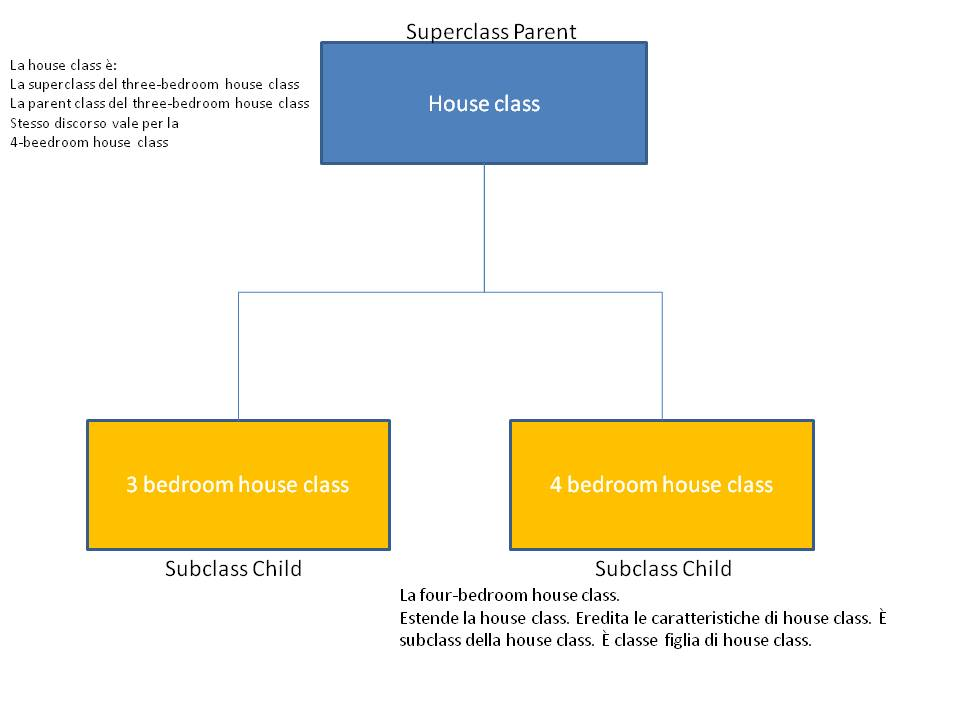
\includegraphics[scale = 0.5]{images/superclass.jpg}
\end{frame}

\section*{Installazione di Java}
\begin{frame}
\begin{block}{}
\begin{center}
\alert{\large{INSTALLAZIONE}\\}

\includegraphics[scale=0.7]{images/instJava.jpg}
\end{center}
\end{block}
\end{frame}
\begin{frame}
\begin{block}{Prerequisiti}
Per installare la \textCl{Java Development Kit (JDK)} non sono richieste grosse prestazioni da parte della macchina.
Unico prerequisito è avere i permessi anche di amministratore della macchina in quanto verranno modificate le variabili
d'ambiente.
\end{block}
\begin{block}{}
Verrà spiegato un metodo per installare la JDK per sistemi windows. Per chi utilizza \textCl{Linux o Mac OsX} posso dare dei 
consigli in privato. In linea di massima chi utilizza linux e mac comunque deve avere i permessi di amministratore della
macchina.
\end{block}
\end{frame}

\begin{frame}
\begin{block}{}
\begin{enumerate}
\item Andate sul sito: \texttt{\footnotesize{http://www.oracle.com/technetwork/java\\/javase/downloads/index.html}} 
dove scaricherete la versione Standard Edition. Effettuate anche il download della documentazione di Java;
\item Double-click sulla icona della JDK;
\item Tra le varie features che ti permette di installare assicuratevi che sia selezionato
\begin{itemize}
\item Development tools;
\item Public Java Runtime Enviroment.
\end{itemize}
\end{enumerate}
\end{block}
\end{frame}
\subsection*{Variabile d'ambiente 1}
\begin{frame}
%\begin{block}{Modifica delle variabili d'ambiente \textbf{PATH}}
La variabile d'ambiente PATH specifica un elenco di directory separate da punto e virgola ";" in cui il sistema ricerca i file eseguibili (nell'ordine in cui sono indicate), oltre che nella directory corrente.
%\end{block}
%\begin{block}{}
\begin{figure}
\begin{center}
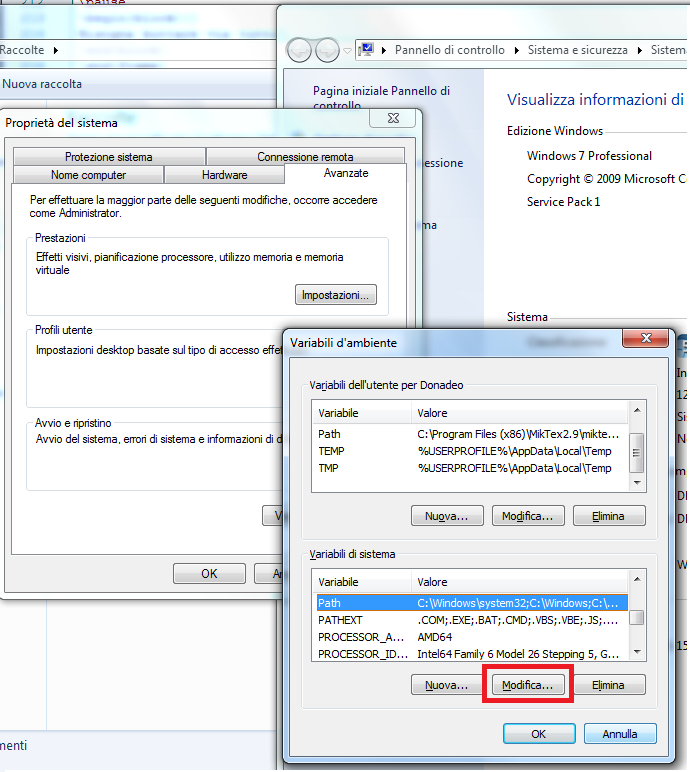
\includegraphics[scale=0.3]{images/path1.png}
\caption{\footnotesize{Tasto destro su computer-$>$Proprietà-$>$Impostazioni avanzate di sistema-$>$Avanzate}}
\end{center}
\end{figure}
%\end{block}
\end{frame}

\subsection*{Variabile d'ambiente 2}
\begin{frame}
\begin{figure}
\begin{center}
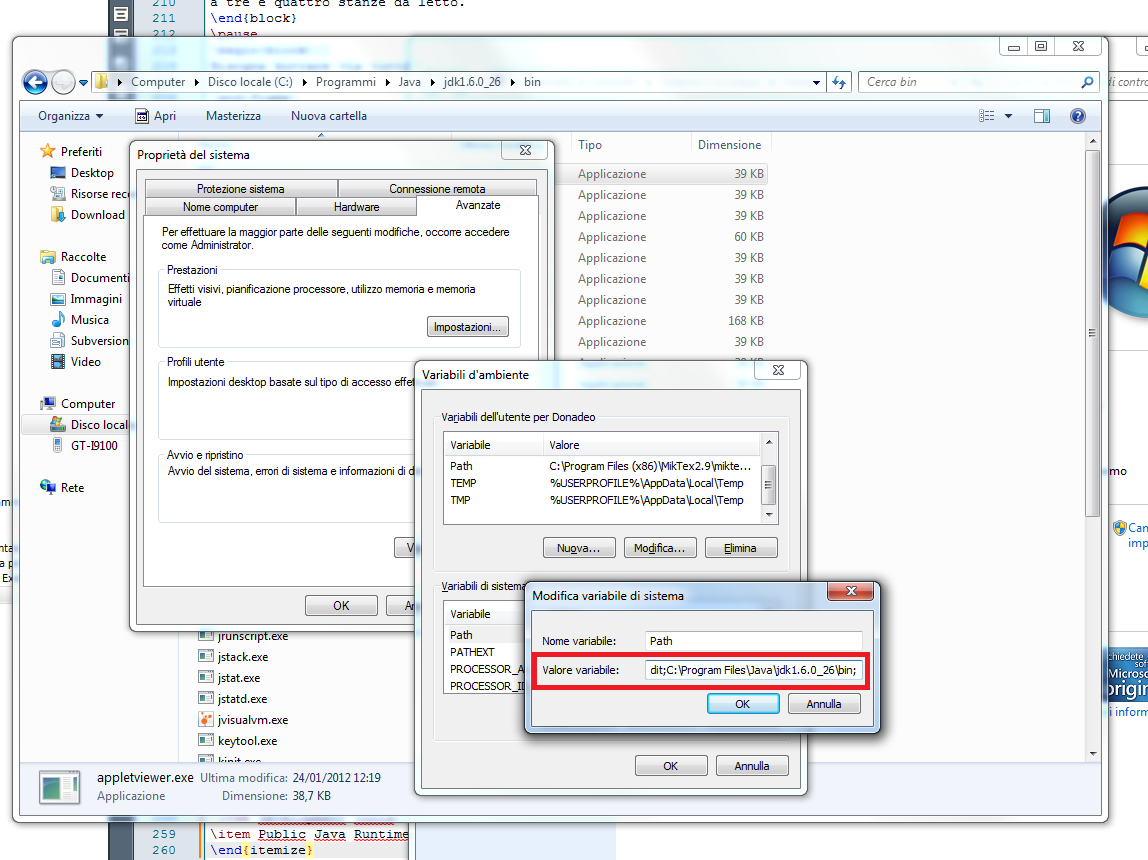
\includegraphics[scale=0.3]{images/path2.png}
\caption{\footnotesize{Aggiungete alla fine il percorso dove avete installato la vostra JDK. Solitamente è:
C:/Programs Files/Java/jdk\_ version/bin}}
\end{center}
\end{figure}
\end{frame}

\subsection*{Documentazione}
\begin{frame}
\begin{block}{}
Un altro dei punti di forza di JAVA è la documentazione. Create una cartella \textCl{docs} all'interno della cartella 
principale di Java. Solitamente \texttt{C:/Programs Files/Java/jdk version/docs}. E fate un unzip della documentazione
che avete scaricato qua. Cliccate su index.html e avrete:
\end{block}
\begin{figure}
\begin{center}
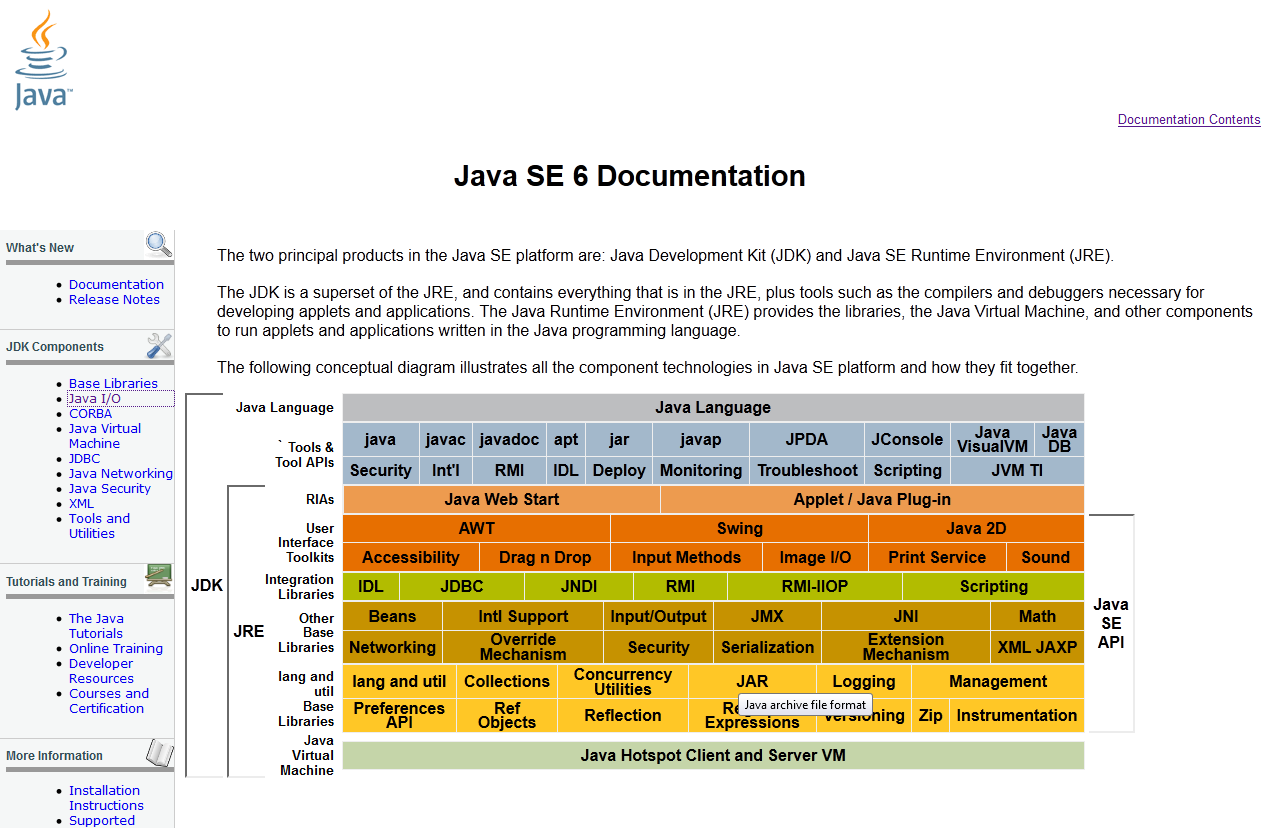
\includegraphics[scale=0.2]{images/doc.png}
\caption{\footnotesize{Documentazione Java. Troverete le API e la spiegazione di tutte classi già messe a disposizione da 
SUN.}}
\end{center}
\end{figure}
\end{frame}

\section{IDE}
\subsection*{Integrated development environment}
\begin{frame}
\begin{block}{IDE}
Un \textit{integrated development environment} IDE (altre si conosciuto come: \textit{integrated design environment, integrated 
debugging environment o interactive development environment}) è un'applicazione che aiuta e facilita gli sviluppatori a 
scrivere del codice. Un IDE normalmente consiste in:
\begin{itemize}
\item Un editor di testo
\item Un compilatore e/o un interprete
\item Un tool che permetta di costruire in maniera automatica un eseguibile
\item Un debugger.
\end{itemize}
\end{block}
\end{frame}

\begin{frame}
\begin{block}{}
Esistono vari IDE che possono aiutare alla progettazione del proprio software.
\end{block}
\begin{figure}
\begin{center}
\begin{minipage}{0.4\textwidth}

\includegraphics[scale = 0.3]{images/geany.png}
\caption{Geany - http://www.geany.org/}
\end{minipage}
\begin{minipage}{0.4\textwidth}

\includegraphics[scale=0.3]{images/netbeans.jpg}
\caption{NetBeans - http://netbeans.org/}
\end{minipage}
\end{center}
\end{figure}
\begin{figure}
%\begin{minipage}{0.2\textwidth}
%\centering

\includegraphics[scale=0.3]{images/eclipse.jpg}
\caption{Eclipse - http://www.eclipse.org/}
%\end{minipage}
\end{figure}
\end{frame}

\section{Il nostro primo programma}
\subsection{Le fasi della programmazione}
\begin{frame}{}
\begin{block}{Le fasi della programmazione}
La scrittura di un programma possiamo dire che si divide principalmente in 3 fasi:
\begin{itemize}
\item scrittura del programma (codice \textCl{sorgente})
\item compilazione del codice sorgente che porta quindi alla creazione del codice \textCl{eseguibile}
\item esecuzione del programma.
\end{itemize}
\end{block}
\begin{block}{Individuare il compilatore Java}
Esistono vari modi per compilare i programmi in Java: internamente all'IDE, utilizzando i comandi da tastiera con l'ausilio di una console (\textbf{è questo il nostro caso}) o tramite delle icone sullo schermo.
\end{block}
\end{frame}
\begin{frame}
\begin{block}{cmd.exe}
Utilizzando il prompt dei comandi di Windows, grazie alle variabili d'ambiente, consente di compilare ed eseguire i programmi 
che verranno scritti in Java. Ecco alcuni comandi utili per utilizzare:
\begin{itemize}
\item Per aprire il prompt dei comandi di Windows è possibile digitare all'interno di cerca \textCl{cmd.exe} o si può trovare 
un collegamento dell'applicazione all'interno di Programmi/Accessori/Prompt dei comandi.
\item \alert{cd} nome cartella: permette di accedere alla cartella.
\item \alert{dir} restituisce un elenco delle cartelle presenti all'interno della cartella di cui si lancia il comando.
\item \alert{cd ..} ritorna alla cartella precedente.
\end{itemize}
\end{block}
\pause
P.S. \textit{Se premete il tasto tab la console completerà la parola permettendovi di risparmiare tempo}
\end{frame}

\begin{frame}
\begin{block}{Cos'è la compilazione}
La compilazione del \textit{codice sorgente} di un programma consente di creare un particolare tipo di formato
di codice eseguibile, detto \textbf{bytecode} che è il codice interpretato dalla Java Virtual Machine
\textit{JVM}.
\end{block}
\begin{block}{}
\begin{itemize}
\item \texttt{javac NomeFile.java }
\end{itemize}
effettua la compilazione del programma, e genera il file \textCl{NomeFile.class}
\end{block}
\begin{block}{}
\textit{Il file che contiene il \textCl{bytecode} è una traduzione delle istruzioni in un linguaggio che la macchina
interpreterà}
\end{block}
\end{frame}
\begin{frame}
\begin{figure}
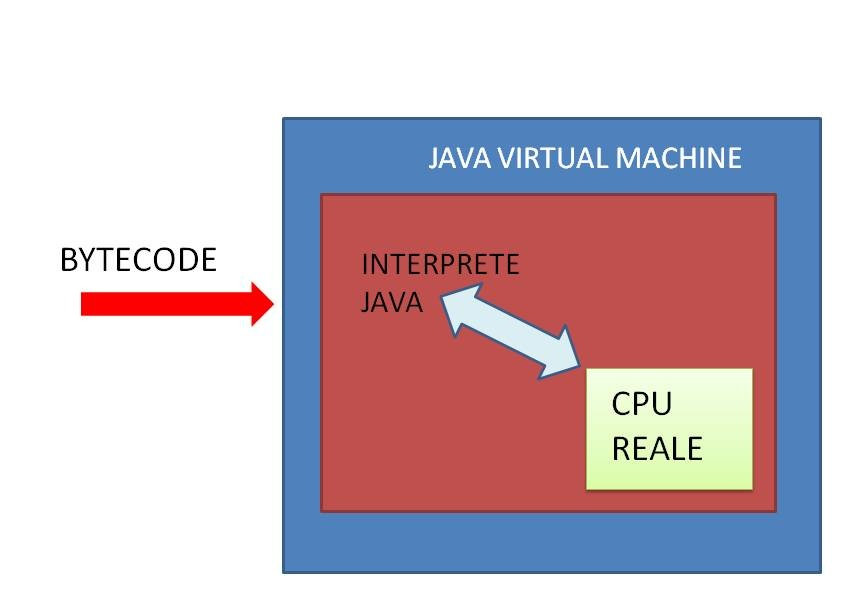
\includegraphics[scale=0.4]{images/jvm.jpg}
\end{figure}
\begin{block}{}
Per \textCl{eseguire} un programma si usa l'\textit{interprete} JAVA, un programma eseguibile sul computer dell'utente.
\end{block}
\end{frame}
\begin{frame}
\begin{block}{}
\begin{itemize}
\item Per poter interagire con il \textit{prompt} è necessario interagire con il sistema operativo, un'operazione di basso
livello che richiede conoscenze specifiche.
\item Queste operazioni, sono state già realizzate dagli autori del linguaggio, che hanno scritto delle classi apposite (ad esempio: \texttt{System}). 
\item Il bytecode di queste classi si strova all'interno delle \textCl{librerie standard}, che sono raccolte di classi.
\end{itemize}
\end{block}
\end{frame}
\begin{frame}
\frametitle{Il processo di programmazione JAVA}
\begin{center}
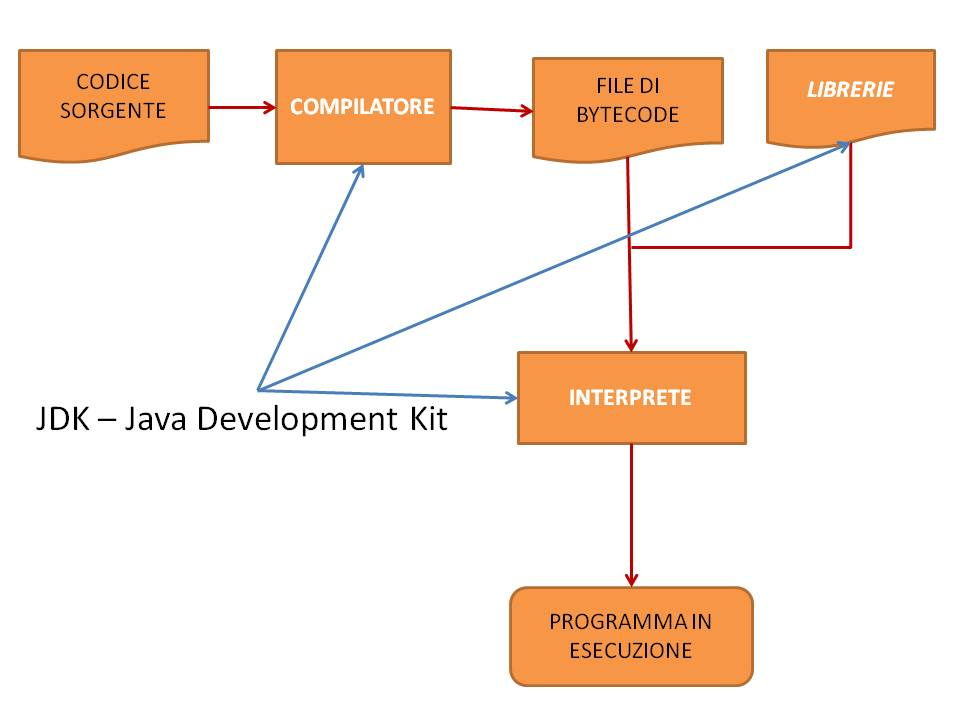
\includegraphics[scale=0.4]{images/processo.jpg}
\end{center}
\end{frame}

\subsection{Hello World}
\begin{frame}
\frametitle{Parlando nel linguaggio Java}
\begin{block}{}
Il linguaggio di programmazione Java, ha tutti gli aspetti di una lingua normale ad esempio come l'Italiano. Java
ha una sua grammatica, nomi comunemente utilizzati e cose di questo genere.
\end{block}
\begin{block}{}
I creatori di Java hanno pensato di dividerlo in due parti. Come l'italiano ha la sua grammatica e nomi comunemente utilizzati
il linguaggio di programmazione Java ha le sue specifiche (\textCl{la sua grammatica}) e Application Programming Interface
(\textCl{parole comunemente utilizzate}).
\end{block}

\end{frame}
\begin{frame}
\begin{block}{}
Tradizionalmente, il primo programma che si scrive quando si impara un linguaggio di programmazione ha il compito di 
visualizzare a schermo il messaggio:
\begin{center}
\large{\alert{Hello, World!}}
\end{center}
\end{block}
\begin{block}{}
Aprite l'editor di testo, Geany, installato sul vostro computer, e salviamo il nostro primo documento
\textCl{HelloWorld.java}.
\end{block}
\end{frame}

\begin{frame}[fragile]
\frametitle{HelloWorld.java}
%\lstset{frame=shadowbox, rulesepcolor=\color{blue}}
\begin{lstlisting}
class HelloWorld{
    public static void main(Strings[] args){
        //Visualizza il messaggio sullo schermo
        System.out.println("Hello, World");
    }
}
\end{lstlisting}
\begin{block}{Attenzione}
\begin{itemize}
\item maiuscole e minuscole sono considerate distinte
\item il file \alert{deve} chiamarsi \textCl{HelloWorld.java}
\end{itemize}
\end{block}
%\end{block}
\end{frame}

\begin{frame}
\begin{itemize}
\item A questo punto compiliamo il nostro primo programma: 
\begin{itemize}
\item Prompt dei comandi
\pause
\item \textCl{cd} Con il percorso per arrivare alla cartella contente il file \texttt{HelloWorld.java}
\pause
\item \alert{javac HelloWorld.java}
\pause
\item se non ci sono errori il compilatore genera il file \textCl{HelloWorld.java}
\end{itemize}
\pause
\item Ora \textbf{eseguiamo} il nostro primo programma:
\begin{itemize}
\item \alert{java HelloWorld}
\end{itemize}
\end{itemize}
\pause
Ottenuto qualcosa sullo schermo?
\end{frame}

\section*{Analisi del primo programma Java}
\begin{frame}[fragile]
\frametitle{Analisi del progrmma Java}
\begin{block}{La prima riga}
La prima riga:
\begin{lstlisting} 
public class HelloWorld 
\end{lstlisting}
definisce una nuova \textbf{classe}.
\begin{itemize}
\item Come abbiamo definito prima le classi rappresentano un concetto fonamentale in Java.
\item Per il momento, consideriamo gli oggetti come \textbf{elementi da manipolare in un programma Java}.
\end{itemize}
\end{block} 
\end{frame}
\subsection*{Analisi del primo programma}
\begin{frame}
\begin{block}{}
\begin{itemize}
\item \textbf{parola chiave} \alert{public} indica che la classe \texttt{HelloWorld} può essere utilizzata da tutti
\item Una \textit{parola chiave} è una parola riservata e che non può essere usata per altri scopi.
\item Ciascun file sorgente può contenere una sola classe pubblica il cui nome deve coincidere con il nome del file.
\end{itemize}
\end{block}

\begin{block}{}
\begin{itemize}
\item Le nostre classi per ora conterranno solo dei \textCl{metodi}
\item Un metodo serve a definire una sequenza di istruzioni che servono per descrivere come svolgere un determinato
compito
\item Un metodo \alert{deve} inserito all'interno di una classe, quindi le classi rappresentano il meccanismo principale di organizzazione dei programmi.
\end{itemize}
\end{block}
\end{frame}

\begin{frame}[fragile]
\begin{lstlisting}
public static void main(Strings[] args){...}
\end{lstlisting}
\begin{block}{main}
con la riga di sopra viene definito il metodo \alert{main}.
\begin{itemize}
\item Un'applicazione Java \textbf{deve} avere un metodo \alert{main}.
\item \texttt{static} significa il che il metodo \alert{main} \textbf{esamina e non modifica gli oggetti 
della classe \texttt{HelloWorld} a cui appartiene}
\end{itemize}
\end{block}
\end{frame}

\begin{frame}
\begin{block}{Commenti}
Nel programma sono presenti anche dei \textbf{commenti} che vengono \alert{ignorati} dal compilatore, ma che rendono
il programma molto più comprensibile.
\end{block}
\begin{block}{}
\begin{itemize}
\item Un commento inizia con la doppia barra \textCl{//} e termina a fine della riga;
\item All'interno del commento può essere scritta qualsiasi cosa; 
\item Se un commento si estende su più righe allora è più comodo farlo iniziare con \textCl{/*} e finire con \textCl{*/}
\end{itemize}
\end{block}
\begin{figure}
\begin{center}
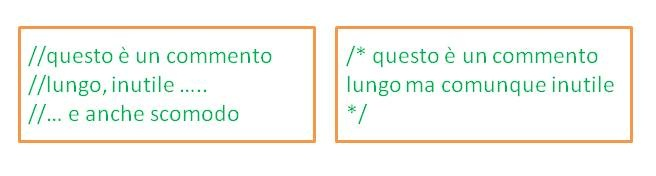
\includegraphics[scale=0.5]{images/commento.jpg}
\end{center}
\end{figure}
\end{frame}

\begin{frame}
\begin{block}{}
Gli enunciati del \textbf{corpo} di un metodo vengono eseguiti uno alla volta \alert{nella sequenza con cui sono scritti}
\end{block}

\begin{block}{}
\begin{itemize}
\item Ogni enunciato termina con il carattere \textbf{\alert{;}} (salvo piccole eccezioni)
\item Il metodo \textCl{main} del nostro esempio ha un solo enunciato che termina con \textbf{\alert{;}}
\end{itemize}
\end{block}

\begin{block}{}
La stringa \textCl{Hello, World} può essere stampata in diverse parti: su un file, sull'\textbf{output\_standard}
o in una finestra. In Java, l'output standard è rappresentato da un oggetto di nome \textCl{out}.
\begin{itemize}
\item come ogni metodo, anche gli oggetti devono essere inseriti all'interno delle classi:
\begin{itemize}
\item \textCl{out} è inserito all'interno della classe \texttt{System} della \alert{libreria standard}.
\end{itemize}
\end{itemize}
\end{block}
\end{frame}

\begin{frame}[fragile]
\begin{lstlisting}
System.out.println("Hello, World");
\end{lstlisting}
\begin{block}{}
Quando si ha un oggetto, bisogna specificare cosa si vuole fare con questo:
\begin{itemize}
\item in questo caso vogliamo \textbf{usare un metodo} dell'oggetto \alert{out}, il metodo \textCl{println} che stampa una riga 
di testo.
\item la coppia di parentesi tonde racchiude le informazioni necessarie per l'esecuzione del metodo (\textbf{parametri})
\end{itemize}
\end{block}
\begin{block}{Il punto}
A volte il carattere \textbf{punto} significa \textit{usa un oggetto di una classe}, altre volte \textit{usa un metodo
di un oggetto}
\end{block}
\end{frame}

\subsection{Invocazione di metodo}
\begin{frame}
\begin{block}{Sintassi}
\begin{center}
\texttt{\textbf{oggetto.nomeMetodo(parametri)};}
\end{center}
\end{block}
\begin{block}{}
\begin{itemize}
\item Viene invocato il metodo \texttt{nomeMetodo} dell'\texttt{oggetto}, fornendo dei \texttt{parametri} se sono richiesti.
\item Se non sono richiesti parametri le parentesi vanno messe ugualmente.
\item se ci sono più parametri questi saranno separati da una \textbf{virgola}.
\end{itemize}
\end{block}
\begin{block}{println}
\begin{itemize}
\item Il metodo \textCl{println} può stampare anche numeri, senza indicare gli apici.
\item C'è anche il metodo \textCl{print}, che funziona come \textCl{println} ma \textbf{non va a capo al termine 
della stampa}.
\end{itemize}
\end{block}
\end{frame}

